%\info{Andrew, Simone}

In this section, we study the sensitivity of the groomed jet mass to variations in the value of $\alpha_s$.
%
We begin with a discussion based on the analytic formulae at LL accuracy.
%
We then perform a PS study, highlighting the interplay between the sensitivity of different parts of the distribution to variations in the value of $\alpha_s$ and NP effects.
%
Finally, we discuss the issue of Casimir scaling and the related issue of using normalized versus unnormalized distributions.


%%%%%%%%%%%%%%%%%%%%%%%%%%%
\subsection{Analytic Understanding}
\label{sec:analytic}
%%%%%%%%%%%%%%%%%%%%%%%%%%%

To get an understanding of the sensitivity of the groomed mass distribution both to the value of $\alpha_s$ as well as to the quark and gluon composition, it is enlightening to study the LL distribution.
%
Here, for simplicity, we consider only the leading logs in the observable, in the resummation region; complete expressions can be found in \Refs{Larkoski:2014wba,Frye:2016aiz,Marzani:2017kqd,Marzani:2017mva}.
%
For $\beta=0$, the LL result at fixed coupling for the cumulative distribution in the resummation region takes the form
%
\begin{align}
\Sigma(\ecf{2}{2})=\exp\left[ - \frac{\alpha_s C_i}{\pi} \log(\zcut) \log (\ecf{2}{2}) \right]\,.
\end{align}
%
This highlights that for $\beta=0$, the groomed jet mass is a single-logarithmic observable, contrasting with the standard double-logarithmic behavior of plain jet mass.
%
Differentiating the cumulative distribution, we obtain the spectrum
%
\begin{align}
\label{eq:ecf_ll_dsitribution}
\ecf{2}{2}  \frac{d\sigma}{d \ecf{2}{2}}=   - \frac{\alpha_s C_i}{\pi} \log(\zcut)   \exp\left[ - \frac{\alpha_s C_i}{\pi}  \log(\zcut) \log (\ecf{2}{2}) \right].
\end{align}
%
Here, we immediately see several interesting consequences.
%
In the resummation region, the slope of the distribution when plotted against $\log\ecf{2}{2}$ is set by the product $\alpha_s C_i$, where $C_i$ is the Casimir factor, namely $C_F = 4/3$ for quarks and $C_A = 3$ for gluons.
%
We therefore see that the groomed mass is indeed sensitive to the value of $\alpha_s$.
%
Due to the larger color charge of gluons, we expect that samples of pure gluon jets would have a significantly higher sensitivity to the value of $\alpha_s$; this expectation will be born out in our parton shower studies below.
%
Because $\alpha_s$ is always multiplied by a color factor, though, knowing the precise quark/gluon composition of a sample is essential, as discussed in \Sec{sec:casimir}.
%
In practice, the parton shower studies and the analytic studies that follow (see \Sec{sec:ben_study}), also include running-coupling corrections \jdt{I think running coupling still respects Casimir scaling. Can someone confirm?} and subleading terms in the splitting function, the later of which violates strict Casimir scaling.


%\gs{I think that here would be a good place to say that the analytic expressions we would use in practice include running-coupling  corrections --- which violate the strict Casimir scaling --- in which the $e_\alpha$ distribution is expressed as a function of  $\alpha_s(p_tR)$.  And this is what will be used in the studies done in Section~5.}

%Should try to get to the point where we can say something about where the sensitivity in the distribution comes from (e.g. slope in log scale is proportional to $C_F\times \alpha_s$).  At the very least, it would be good to write down the LL (or even NLL) functional form for the angularities that we used (it is in the code we got from Ian (LL) and Gregory (NLL)).  Could also punt this to Sec.~\ref{sec:templates} where we will show the templates (could then just give a ref).
%
%\begin{comment}
%The Soft Drop grooming procedure~\cite{Larkoski:2014wba} takes a jet
%with momentum $p_t$ and radius $R$. It re-clusters its constituents
%using the Cambridge/Aachen (C/A) algorithm \cite{Dokshitzer:1997in,
%  Wobisch:1998wt} and iteratively performs the following steps:
%\begin{enumerate}
% \item it de-clusters the jet into 2 subjets $j \to j_1 + j_2$;
% \item it checks the condition 
%\begin{equation}\label{eq:sd-condition}
%\frac{\min (p_{t1} , p_{t2})}{p_{t1}+p_{t2}} > \zcut \left(
%  \frac{\theta_{12}}{R}\right)^\beta\,;
%\end{equation}
%\item if the jet passes the condition, the recursion stops; if not the
%  softer subjet is removed and the algorithms goes back to step 1 with
%  the hardest of the two subjets. 
% \end{enumerate}
%In the case $\beta=0$ Soft Drop essentially reduces to mMDT~\cite{Dasgupta:2013ihk},
% albeit without any actual mass-drop condition. Moreover, while the
% original MDT~\cite{Butterworth:2008iy} algorithm imposed a cut on the ratio of angular distances
% to masses, a so-called $\ycut$, the mMDT variant instead cuts on
% momentum fractions~\cite{Dasgupta:2013ihk} (see
% e.g. \cite{Dasgupta:2013ihk,Dasgupta:2016ktv} for a comparison
% between $\ycut$ and $\zcut$).
% \end{comment}
%
%Notes (order not meaningful): Plot of the two calculations for softdrop mass?  Show plots of the ATLAS and CMS measurements?  Actually, I'm not sure we can show CMS since it is only preliminary.  Say something about mass versus $k_t$?
%







%%%%%%%%%%%%%%%%%%%%%%%%%%%
\subsection{Parton Shower Study}
%%%%%%%%%%%%%%%%%%%%%%%%%%%

\jdt{We switched notation in this section from $\ecf{2}{\alpha}$ to $e_\alpha$.  I am doing my best to stick with the two-point correlator language we introduced before, eliminating ``angularity''.  The plots have not yet been changed to reflect this, though.  It would also be helpful to increase the font size.  While we're at it, can we have the jet mass direction go in the same way as Figure 3?}

From the point of view of fitting for $\alpha_s$, a good observable is one whose probability distribution changes significantly with variations in $\alpha_s$.
%
However, many observables that significantly change with $\alpha_s$ are also very sensitive to NP effects, such as the constituent multiplicity inside jets.
%
Here, we study many two-point correlators to quantify the tradeoff between the sensitivity to $\alpha_s$ and the robustness to NP effects.

\begin{figure}[t]
\begin{center}
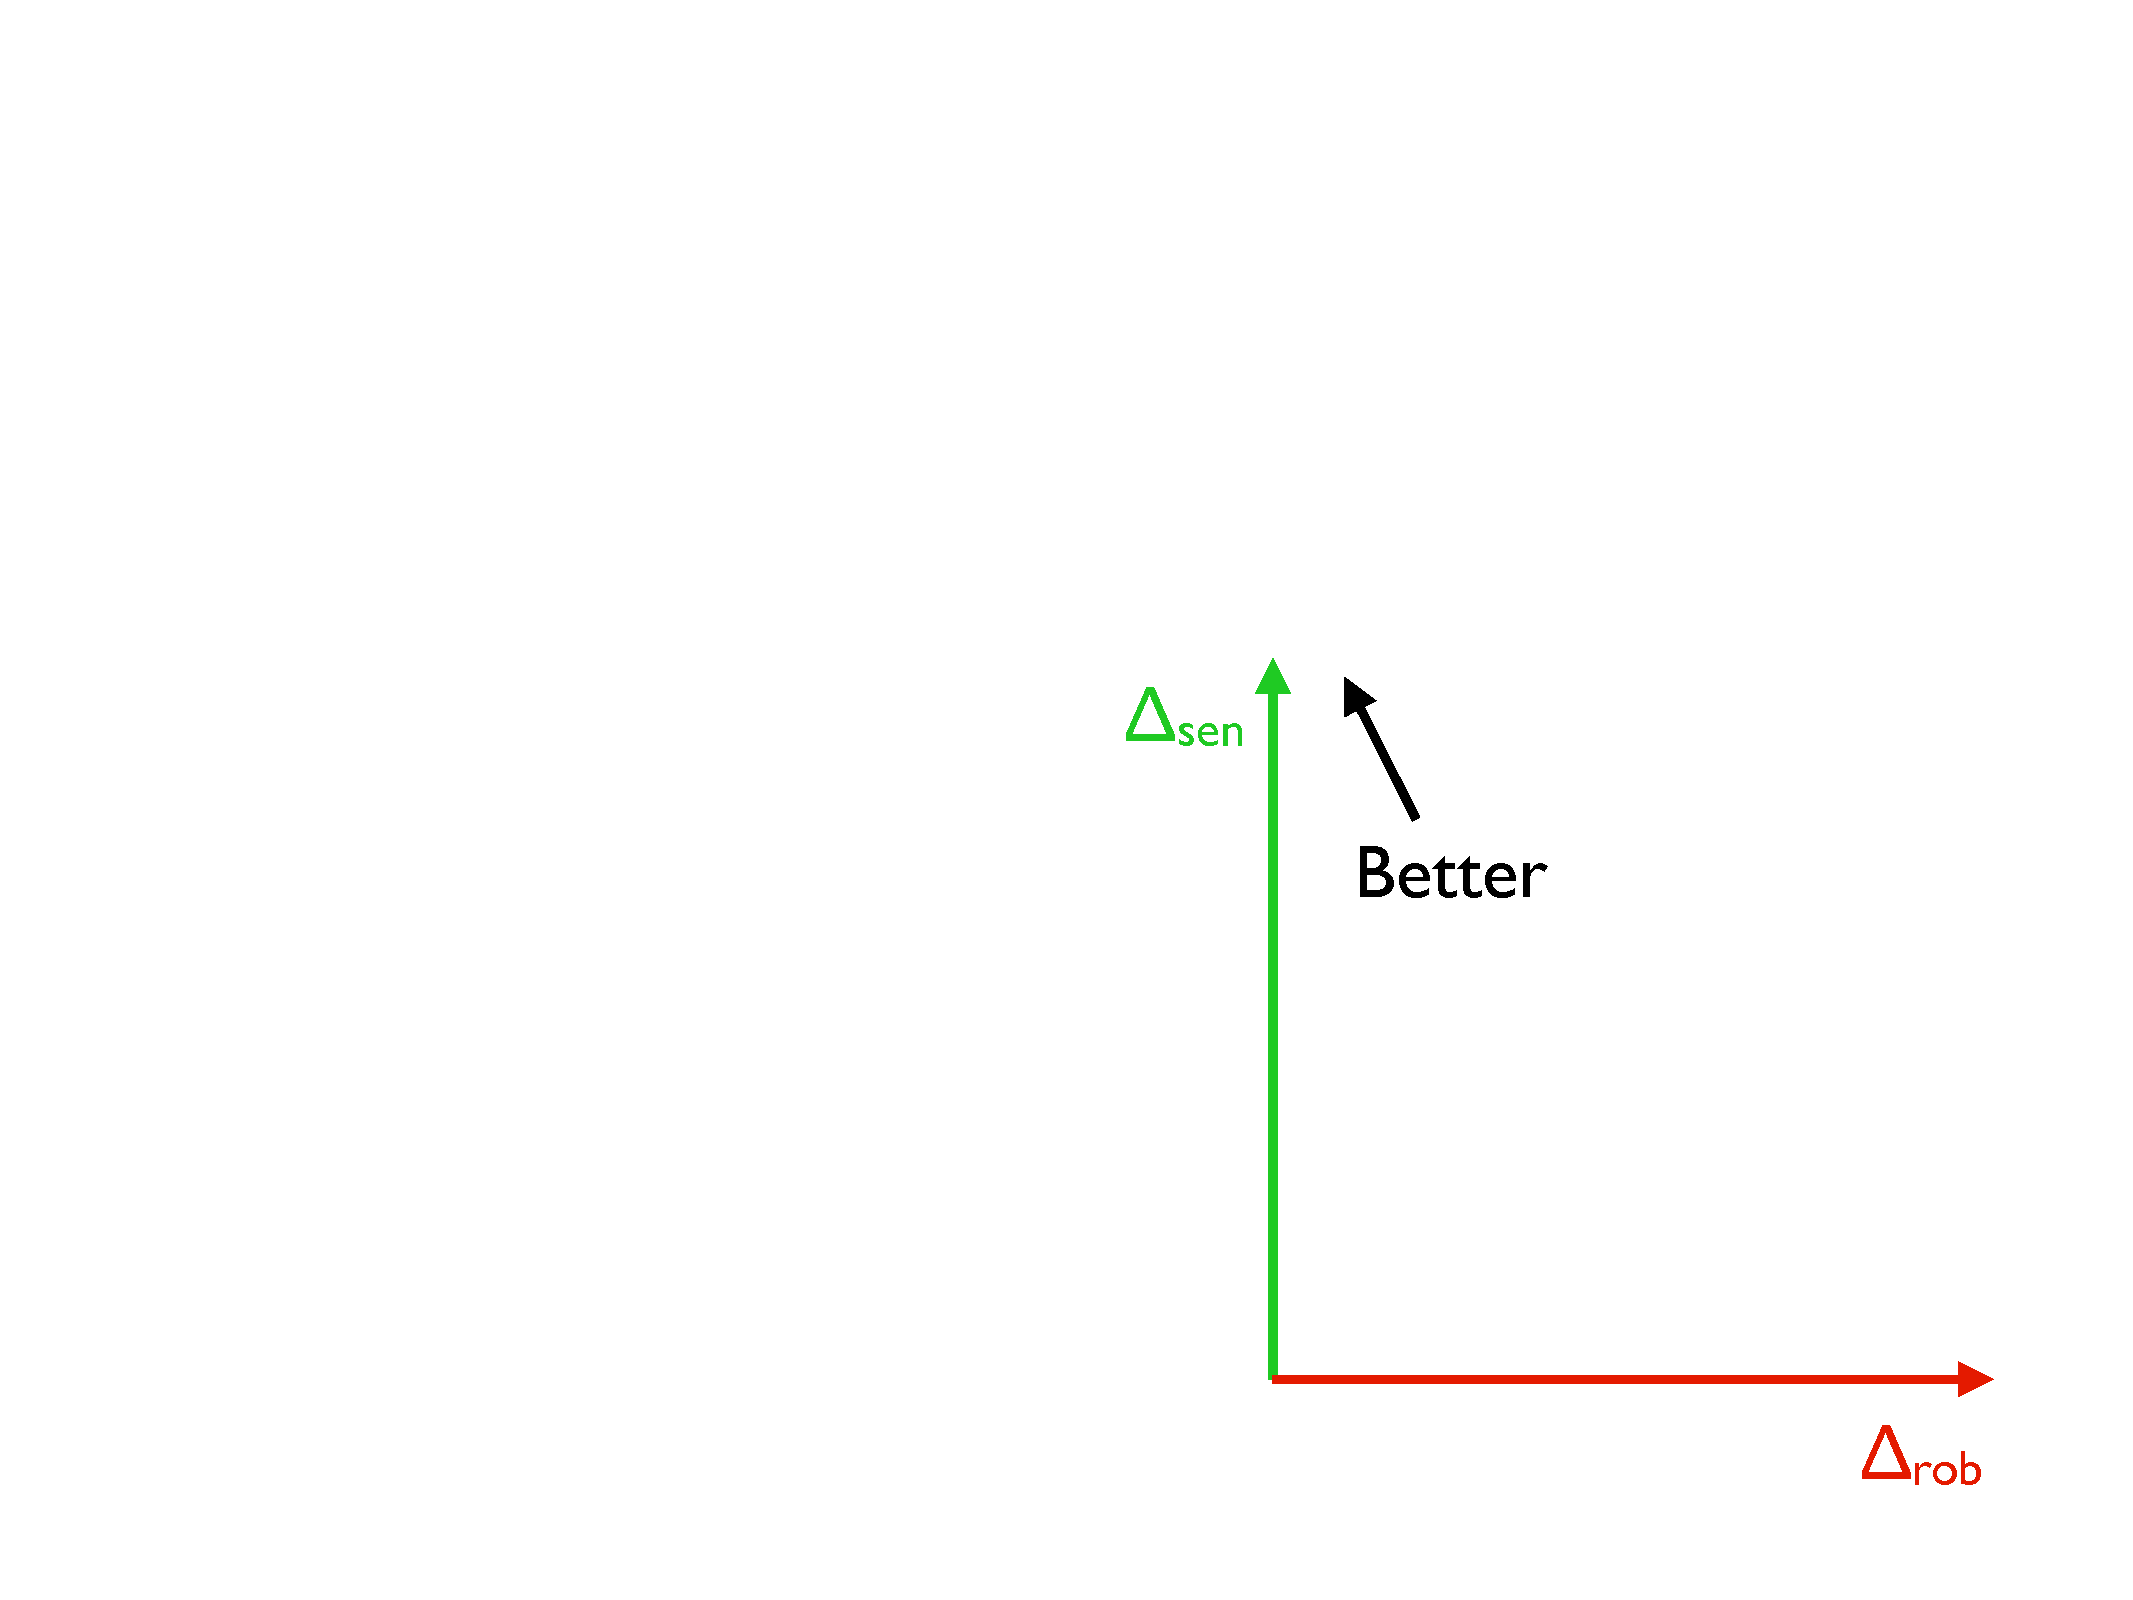
\includegraphics[width = 0.4\columnwidth]{figures/robustnessschematic.pdf}
\end{center}
\caption{A schematic diagram to illustrate the sensitivity-robustness plane defined by the separation power in \Eq{eq:seppower}.}
\label{fig:robustnessschematic}
\end{figure}

Given two probability distributions $f$ and $g$ in some observable $\lambda$, we define the separation power $\Delta(f,g)$~\cite{Harrison:1998yr} as
%
\begin{align}
\label{eq:seppower}
\Delta(f,g)=\frac{1}{2}\int d\lambda \, \frac{(f(\lambda)-g(\lambda))^2}{f(\lambda)+g(\lambda)}.
\end{align}
%
The separation power is a number in $[0,1]$, where $\Delta=0$ if and only if $f=g$.
%
If $f$ is the nominal probability distribution of some observable and $g$ is the distribution of the same observable with a different value of $\alpha_s$, we would like $\Delta(f,g)$ close to 1 (sensitivity).
%
In contrast, if $g$ is the same as $f$ with some variation in the NP effects, then we would like $\Delta(f,g)$ to be close to $0$ (robustness).
%
The plane used to study the tradeoff between sensitivity and robustness is shown in \Fig{fig:robustnessschematic}.
%
Not all information about $\alpha_s$ sensitivity is captured by a single point in \Fig{fig:robustnessschematic}, because sensitivity to NP effects could be in regions of low $\alpha_s$ sensitivity and vice versa.
%
Therefore, it is also useful to study the integrand of \Eq{eq:seppower} as a function of different observables $\lambda$.


This sensitivity-robustness tradeoff is studied using two parton shower generators: \herwig.1~\cite{Bellm:2015jjp,Reichelt:2017hts} with the default tune and \pythia.223~\cite{Sjostrand:2006za,Sjostrand:2014zea} with the tune Monash~\cite{Skands:2014pea} \jdt{My understanding is that we will not have Pythia results, right?}.
%
These programs are formally LL accurate, though they include effects beyond \Eq{eq:ecf_ll_dsitribution}.
%
Results are presented separately for quark and gluon jets, using the $Z+q$ and $Z+g$ hard-scattering processes.
%
A variety of two-point correlators (as defined in \Sec{sec:shape_def}) are studied, with $\alpha\in\{0.5,1.0, 2.0\}$ corresponding to the Les Houches Angularity~\cite{Gras:2017jty}, width, and mass, respectively. 
%
Additionally, various Soft Drop grooming parameters are studied by varying $\beta\in\{0,1,2\}$ and $z_\text{cut}\in \{0.05,0.1,0.2\}$.  

\begin{figure}[t]
\begin{center}
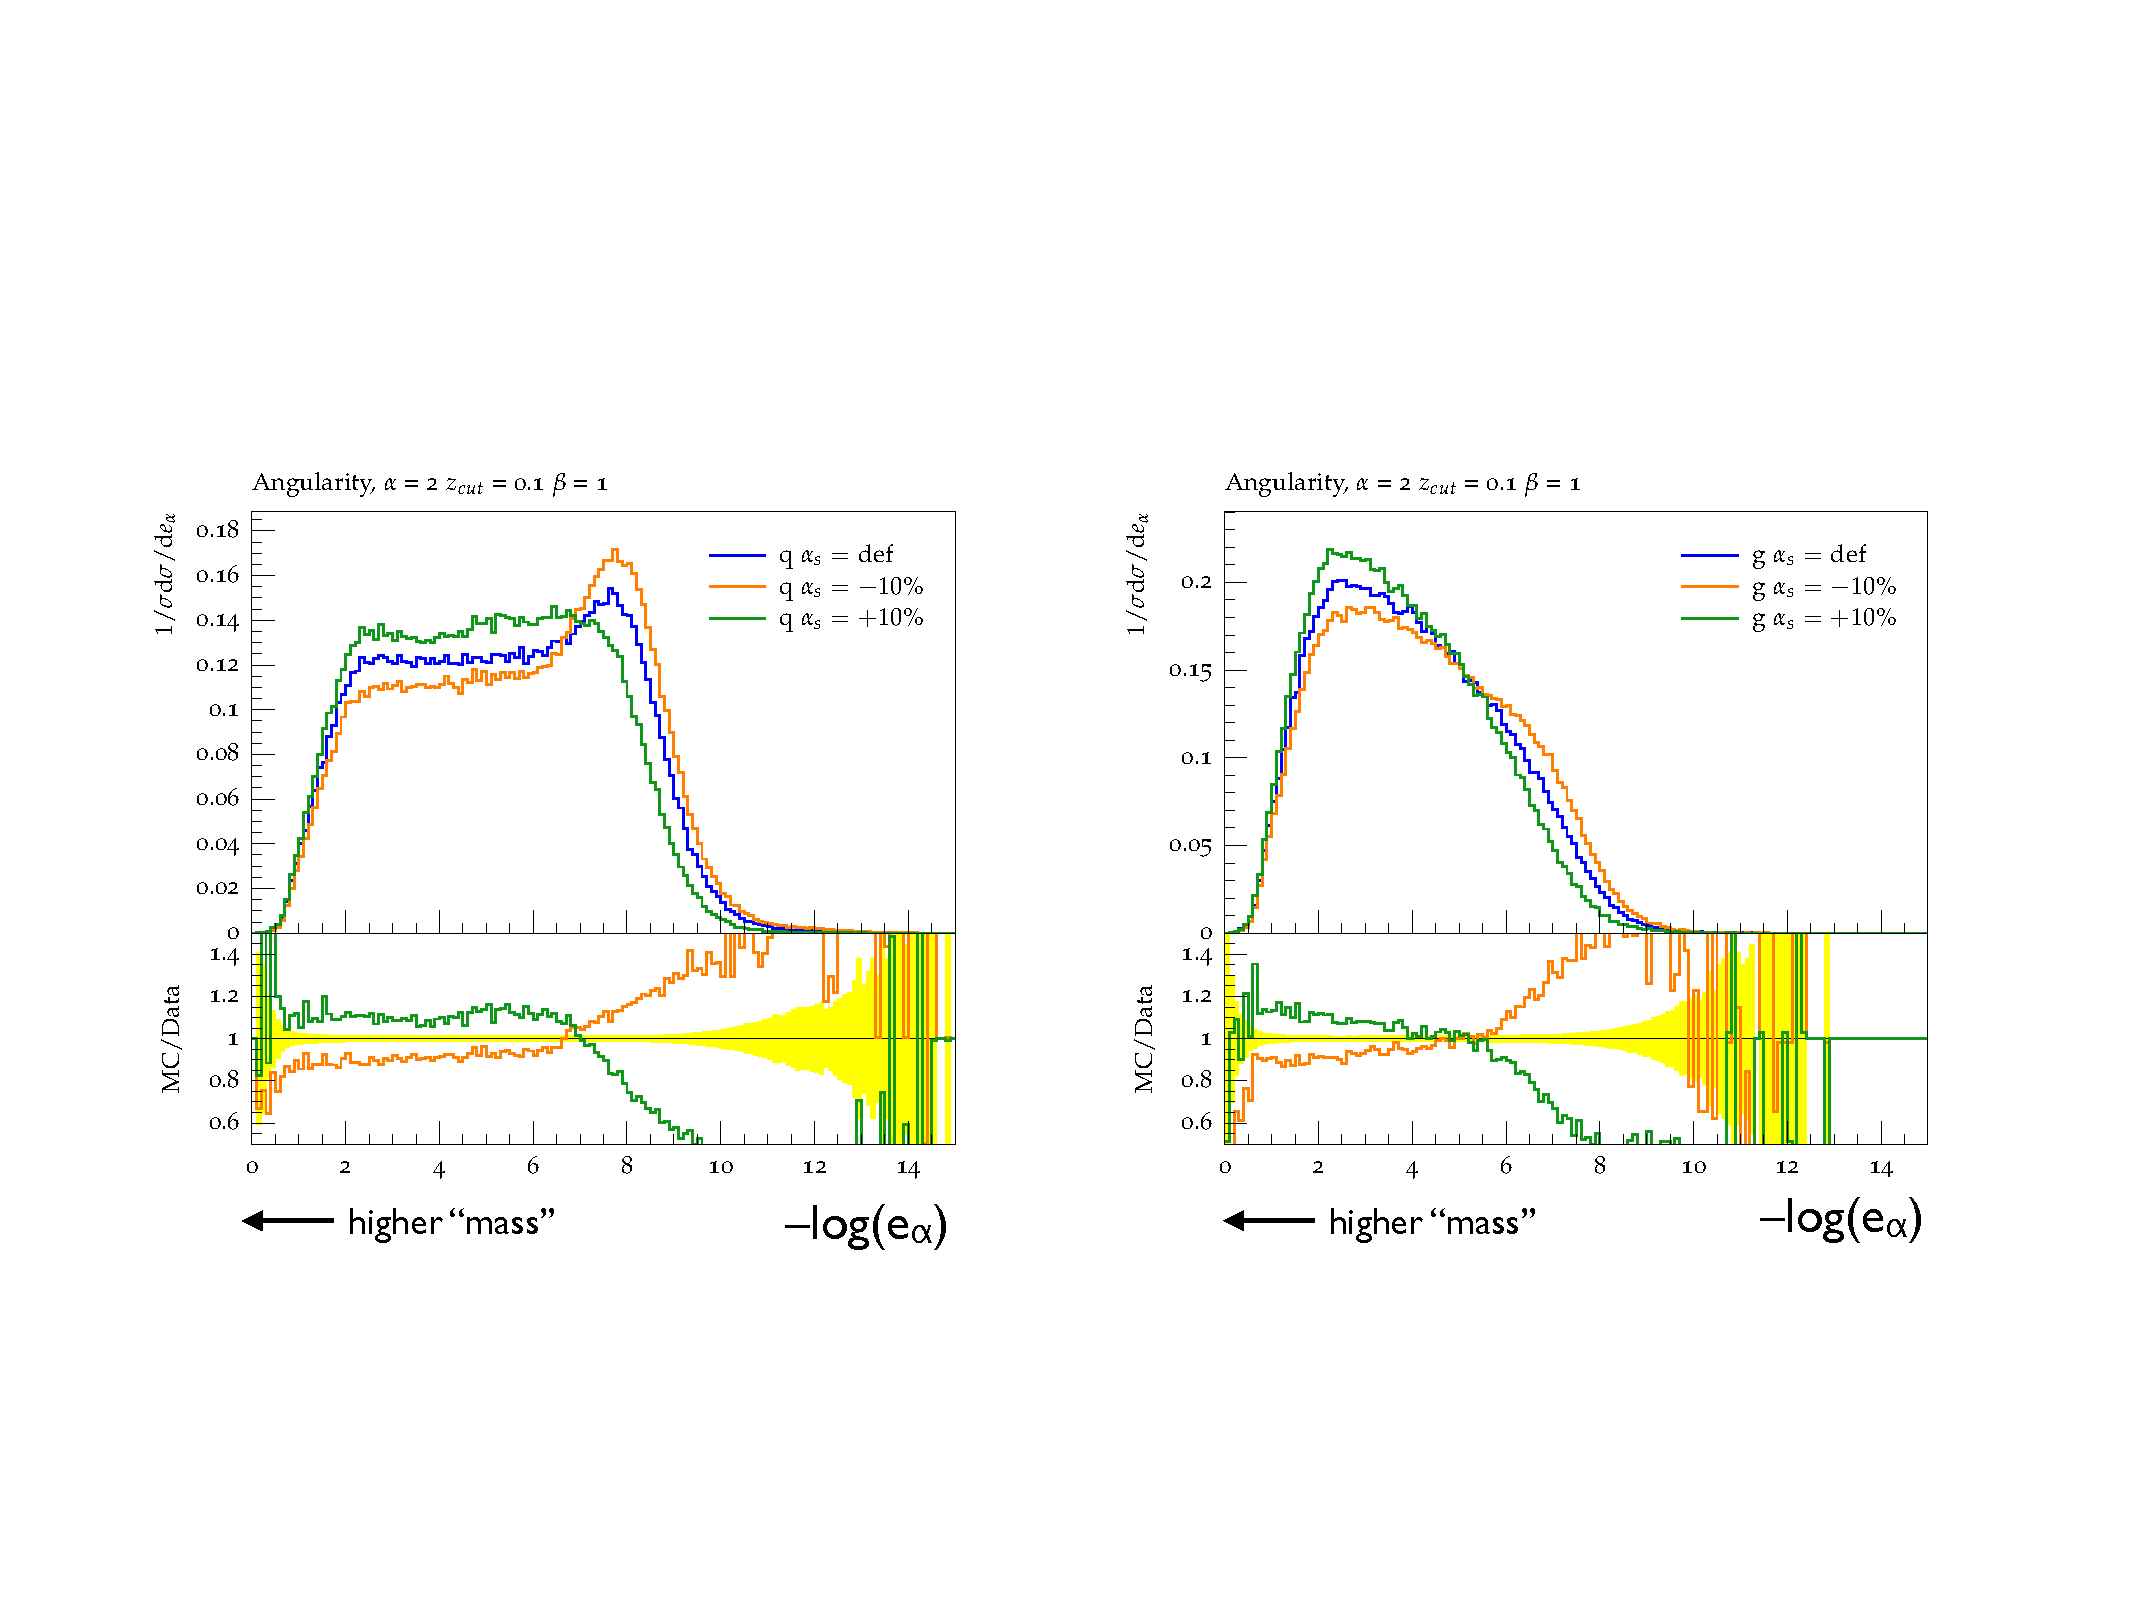
\includegraphics[width = 0.99\columnwidth]{figures/sensitivity.pdf}
\end{center}
\caption{\jdt{From the TODO:  Cut off Fig.~\ref{fig:sensitivity} and Fig.~\ref{fig:robustness} at -12.  Also, add a statement or plot about Pythia.}  The sensitivity to $\alpha_s$ in \herwig.  Shown is the distribution of the normalized squared jet mass ($\ecf{2}{2}$) for quark jets (left) and gluon jets (right), with higher values of the mass are on the left.  The blue line uses $\alpha_s=0.118$ while the green and orange lines have the value of $\alpha_s$ varied by $10\%$.  The lower panels show the ratio with respect to the $\alpha_s=0.118$ curve.}
  %.\textbf{Maybe cut the x-axis at high values?  \gs{Yes, sth like $-\log(e_\alpha)=$11 or 12.}  Maybe comment what the picture looks like for Pythia?}
\label{fig:sensitivity}
\end{figure}

\begin{figure}[t]
\begin{center}
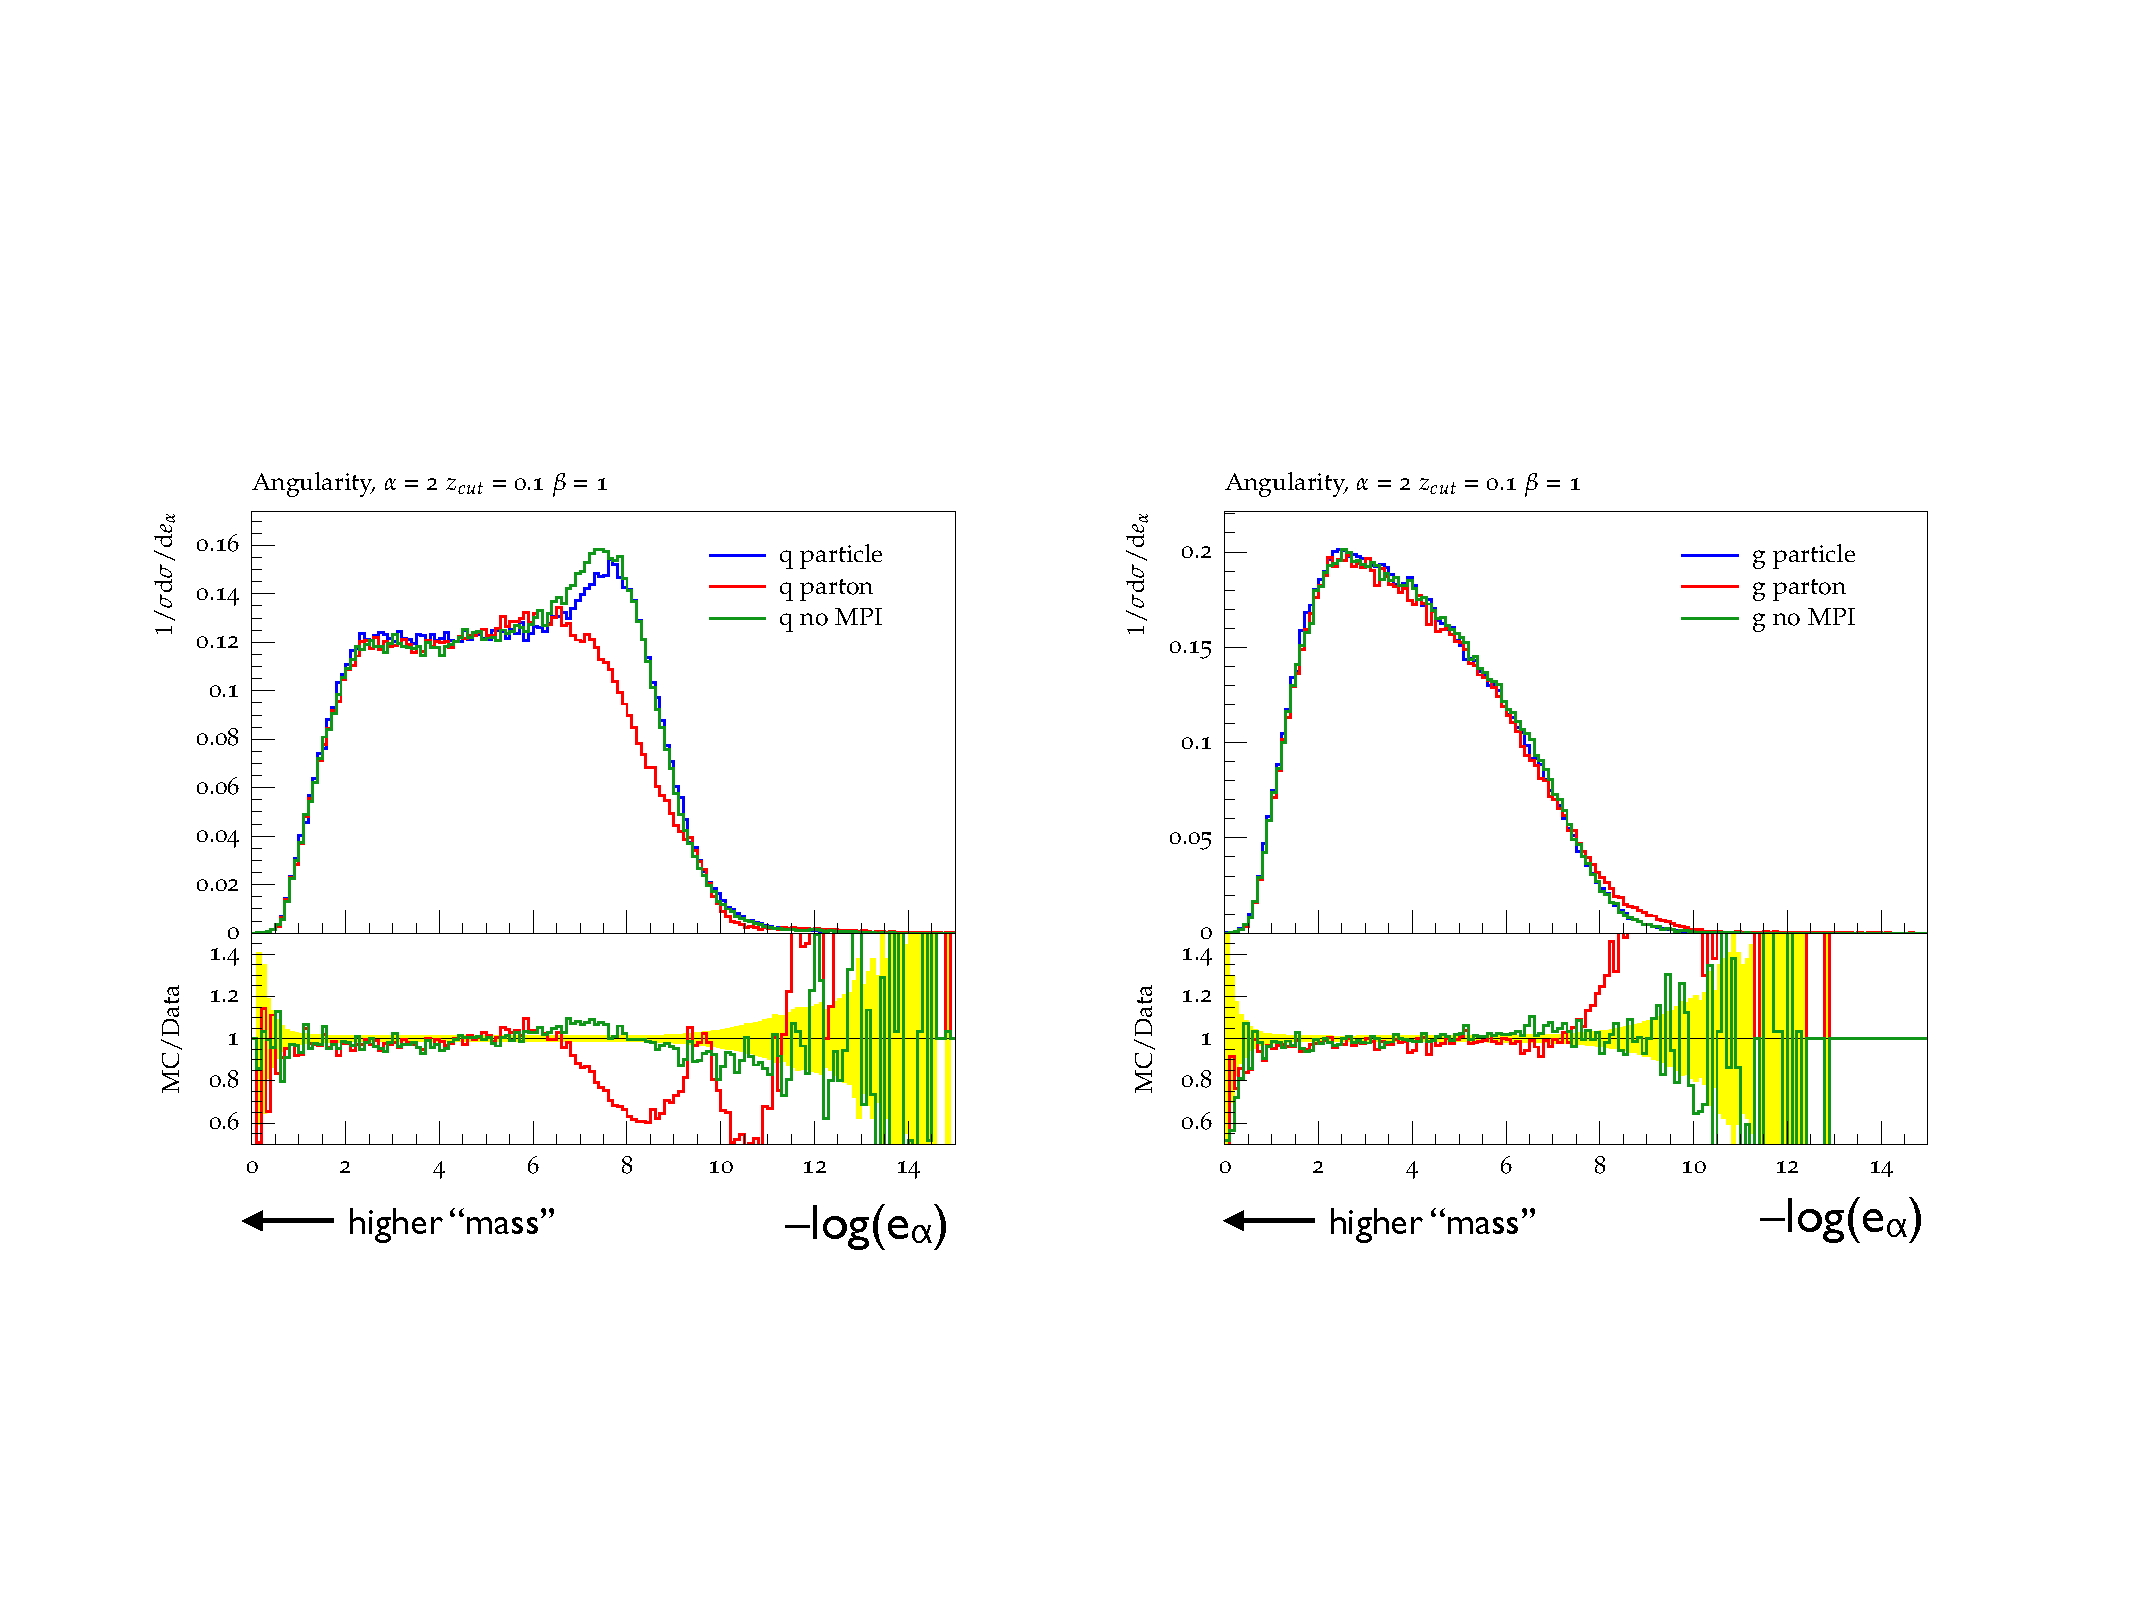
\includegraphics[width = 0.99\columnwidth]{figures/robustness.pdf}
\end{center}
\caption{The robustness to NP effects in \herwig, with the same distributions as \Fig{fig:sensitivity}.
%
The blue line shows the default particle-level simulation that includes the standard cluster hadronization model.
%
The red curve has hadronization turned off and the green curve is the same as the blue, but with the \herwig model for multiple parton interactions (MPI) turned off.
%
MPI is also off for the red curve.}
  % \textbf{Maybe cut the x-axis at high values?  Maybe comment what the picture looks like for Pythia?}
\label{fig:robustness}
\end{figure}

\begin{figure}[t]
\begin{center}
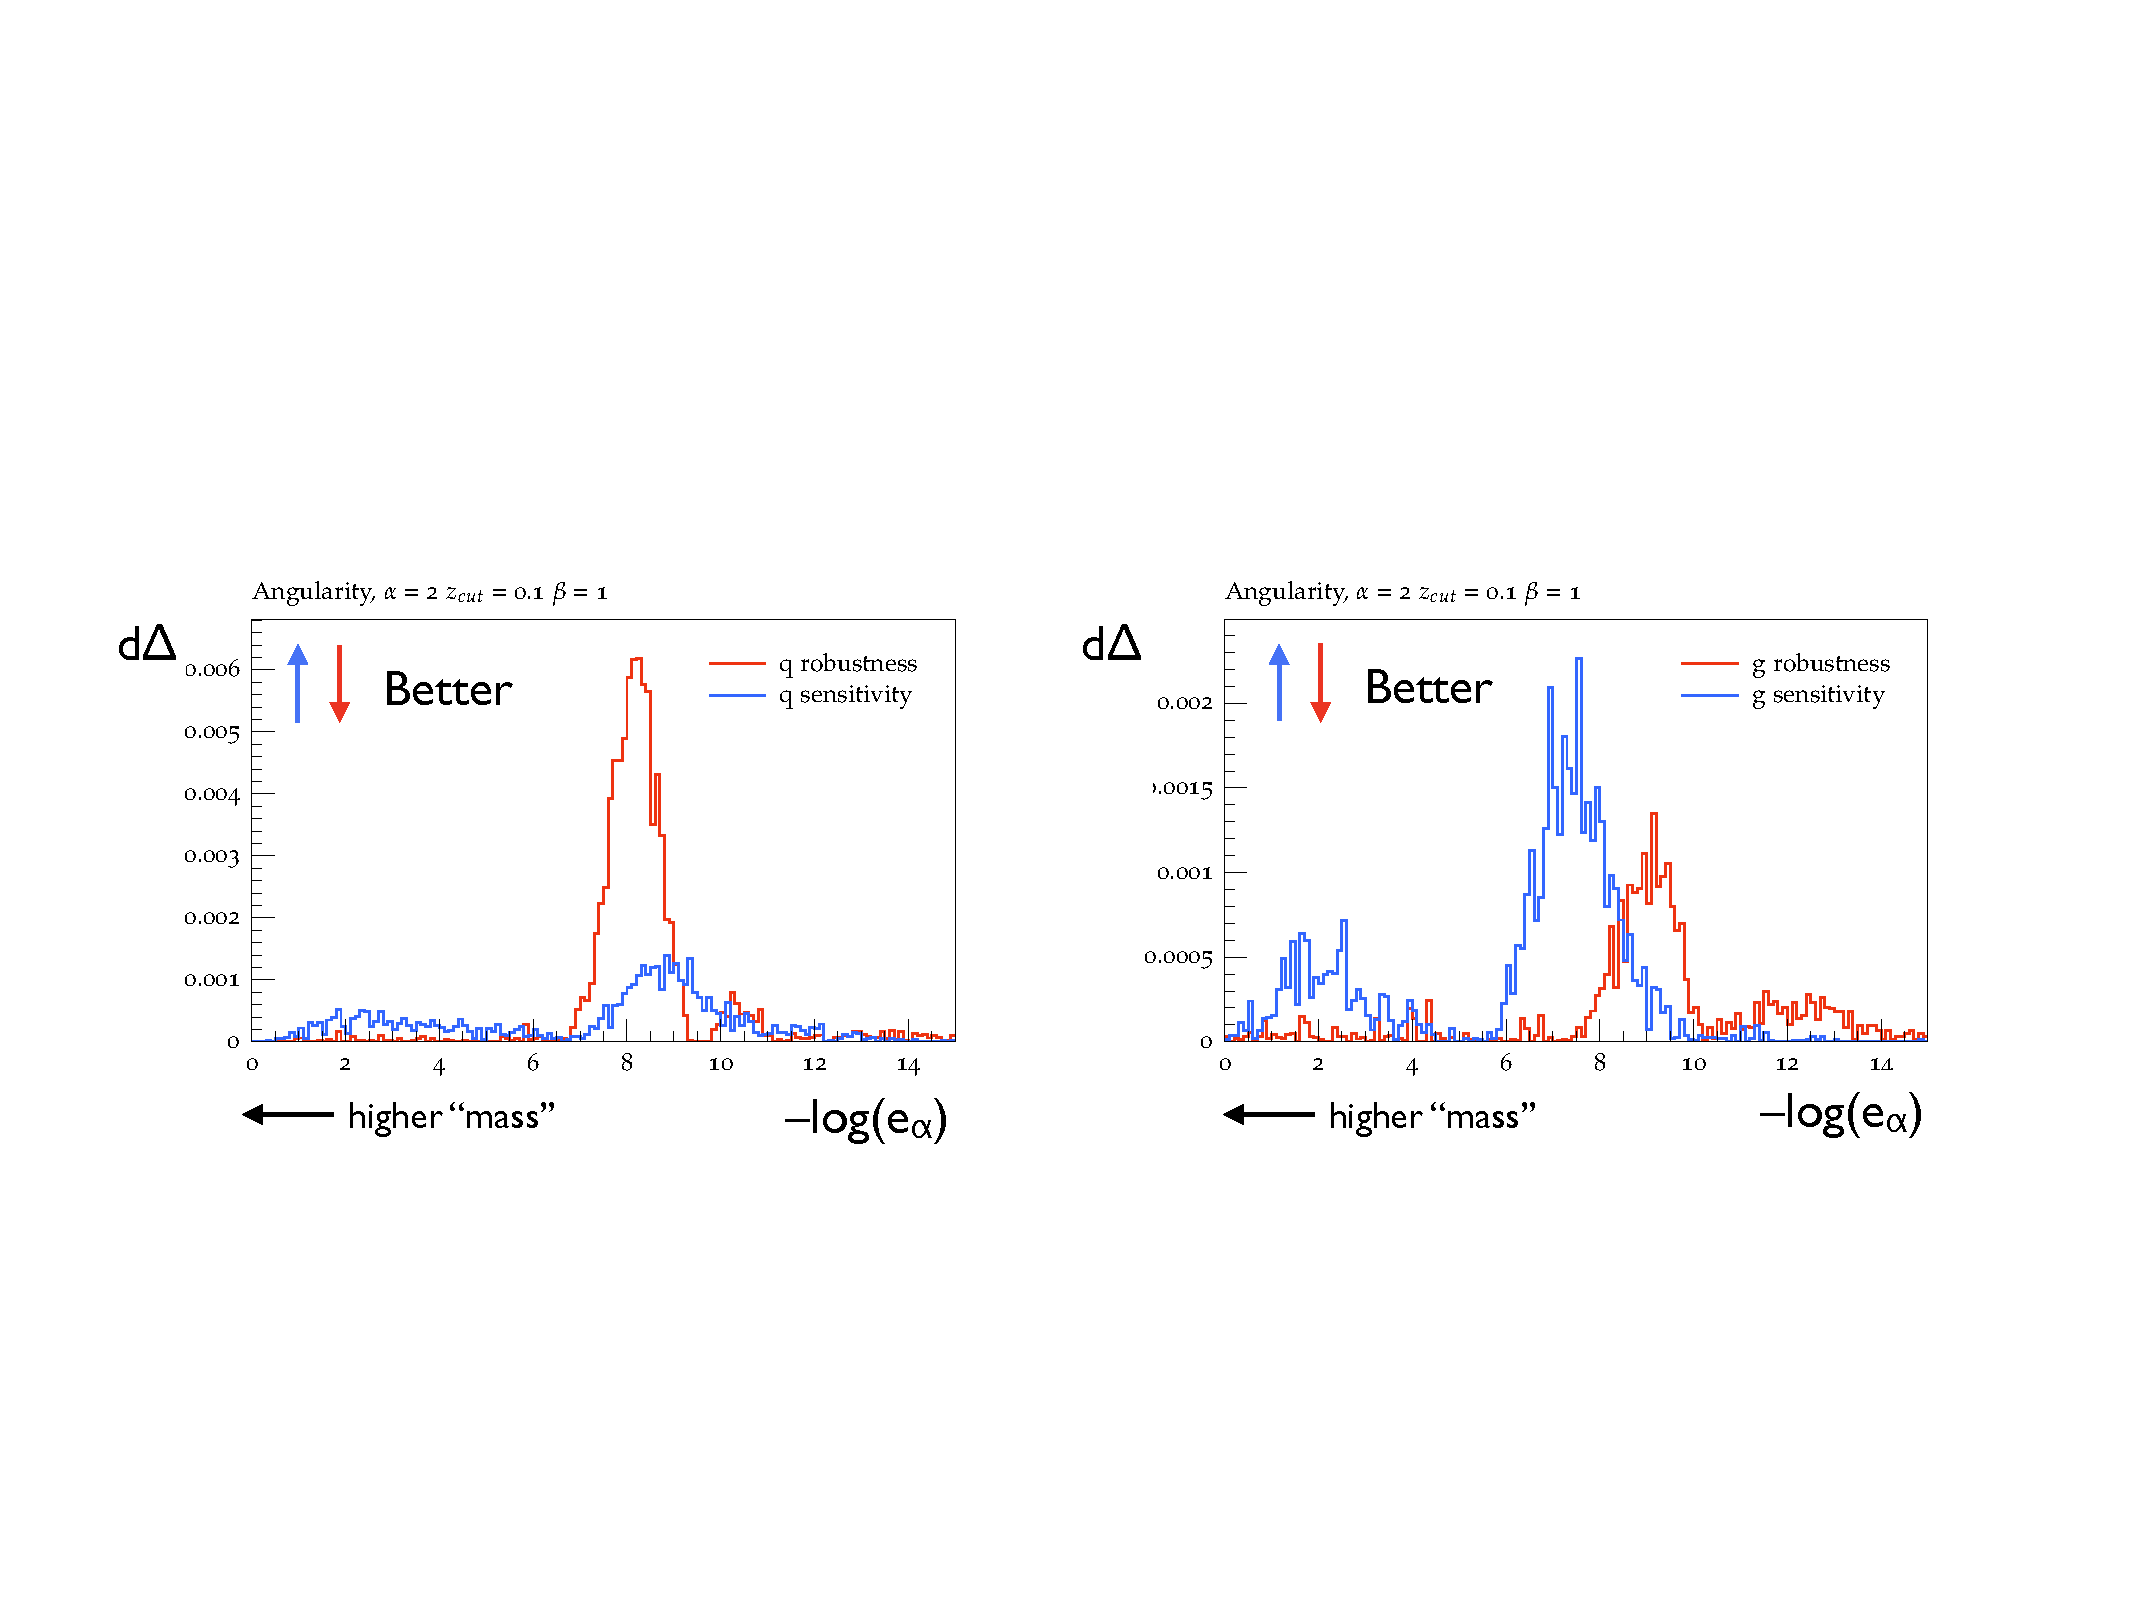
\includegraphics[width = 0.99\columnwidth]{figures/differentialseparation.pdf}
\end{center}
\caption{The integrand of \Eq{eq:seppower} in \herwig.  Shown is the normalized squared jet mass ($\ecf{2}{2}$)  for quark jets (left) and gluon jets (right), with higher values of the mass are on the left.  The baseline $f$ function from \Eq{eq:seppower} is the same for the red and blue curves.  For blue (sensitivity) the $g$ function is from varying $\alpha_s$ by 10\%, whereas for red (robustness) the $g$ function hadronization is turned off.  Note the different vertical scale in the left and right plots. }
\label{fig:differentialseparation}
\end{figure}

The sensitivity to $\alpha_s$ is shown in \Fig{fig:sensitivity}, in the case of normalized squared jet mass ($\ecf{2}{2}$) for quark and gluon jets.
%
To the left of the low-mass NP peak, the shape of the $\ecf{2}{2}$ distribution is nearly flat for quarks and nearly linear (in the log-space) for gluons, as expected from \Eq{eq:ecf_ll_dsitribution}.
%
Increasing $\alpha_s$ shifts the quark distribution up but has nearly no impact on the shape of the distribution below the peak.
%
The size of the NP peak is significantly impacted by the value of $\alpha_s$, with smaller $\alpha_s$ values implying that NP effects are more important to the groomed mass distribution.
%
In contrast, the slope of the distribution for gluons does change with the variations in $\alpha_s$, but there is no low-mass NP peak.

The robustness to NP effects is shown in \Fig{fig:robustness}, using the same $\ecf{2}{2}$ distribution but now with variations in the modeling of hadronization and MPI effects.
%
Overall, there is excellent stability in the $\ecf{2}{2}$ distribution.
%
The low-mass peak for quarks is almost entirely due to hadronization effects.
%
According to \herwig, the impact of hadronization is much smaller for gluon jets, as expected since perturbative effects push the distribution away from the NP-sensitive region in \Eq{eq:np}.

\Fig{fig:differentialseparation} shows the distribution of the differential separation power (integrand of \Eq{eq:seppower}), using the variation with $\alpha_s$ as the sensitivity and the change from turning off hadronization as the robustness.
%
For quark jets, \Figs{fig:sensitivity}{fig:robustness} showed that the biggest variations with $\alpha_s$ occurred at low mass which is also where NP effects are largest.
%
This corresponds to the peak in the blue and red distributions in \Fig{fig:differentialseparation} occurring in nearly the same location.
%
In contrast, the peaks are more well-separated in \Fig{fig:differentialseparation} for gluon jets and the blue is shifted to higher mass values where there is more perturbative control.
%
This suggests that gluon-enriched samples are going to play an important role for $\alpha_s$ determination from jet substructure.

\begin{figure}[t]
\begin{center}
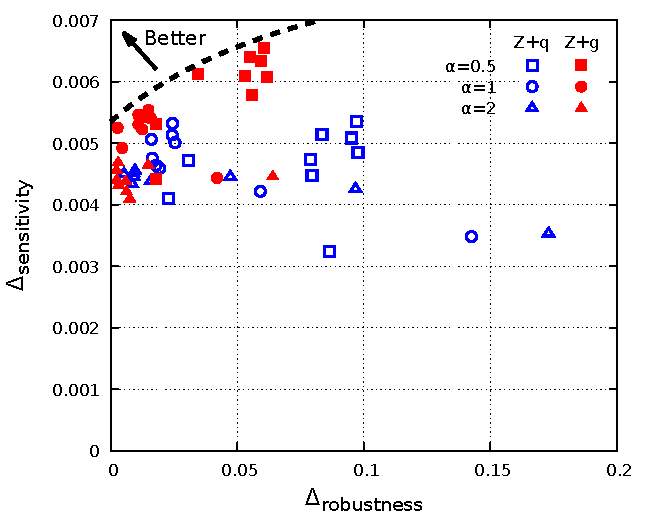
\includegraphics[width = 0.6\columnwidth]{figures/robsep.pdf}
\end{center}
\caption{The tradeoff between sensitivity and robustness for 27 two-point correlator/jet grooming combinations.  Open blue symbols represent quark jets and closed red symbols represent gluon jets.}
\label{fig:robseptradeoff}
\end{figure}

A summary of the sensitivity-robustness tradeoff for many two-point correlators is presented in \Fig{fig:robseptradeoff}.  As already observed for the jet mass, gluons tend to have superior sensitivity and robustness compared with quarks.
%
This is not surprising, as gluons have more perturbative radiation than quarks ($C_A>C_F$).
%
The jet mass has $(\Delta_\text{sensitivity},\Delta_\text{robustness})=(0.097,0.0043)$, $(0.015,0.0046)$ for quarks and gluons, respectively, using $\beta=0$ and $z_\text{cut}=0.1$.
%
The groomed two-point correlators with the best quark and gluon sensitivity and robustness have $\alpha=1$, $z_\text{cut}=0.05$ and $\beta=1$ or $\beta=2$.
%
The choice of $\alpha=1$ correspond to $k_t$ (a.k.a.~width) instead of mass, which may not be so surprising since the scale of $\alpha_s$ is set by $k_t$ and not mass.
%
Interestingly, $k_t$ with $\beta=0$ has significantly worse sensitivity than $\beta=1$ or $\beta=2$, highlighting the importance of having some double-logarithmic information. 
%
This study suggests that $k_t$ observables are important to include in future experimental and theoretical studies.
%
It would also be interesting to study how the robustness versus sensitivity picture changes when considering only subsets of the available observable range.

%%%%%%%%%%%%%%%%%%%%%%%%%%%
\subsection{The Issue of Casimir Scaling}
\label{sec:casimir}
%%%%%%%%%%%%%%%%%%%%%%%%%%%

While we have illustrated that groomed jet mass provides excellent sensitivity to $\alpha_s$, particularly for gluon jets, one problem that is immediately clear from \Sec{sec:analytic} is that the leading behavior of the distributions is always dominated by the product $\alpha_s C_i$.
%
While this is broken at higher perturbative orders, it implies that at lowest order there is a complete degeneracy of the value of $\alpha_s$ and the quark versus gluon fraction of jets.
%
This problem is not faced for dijet event shapes at $e^+e^-$ colliders, which are almost entirely quark dominated.

There are a variety of different approaches to overcome this problem, each with their own advantages and disadvantages.
%
First, the quark and gluon fractions are perturbatively calculable given the parton distribution functions (PDFs).
%
Therefore, perturbatively calculating the quark and gluon fractions inputs the most possible information, and should correspondingly lead to the best sensitivity for $\alpha_s$.
%
This has the downside, however, of also introducing sensitivity to the PDFs, which in principle should be fitted along with $\alpha_s$~\cite{Accardi:2016ndt}.
%
This difficulty also enters into other $\alpha_s$ extractions at the LHC, for example the $3$-$2$ jet rate \jdt{cite needed} or the energy-energy correlator \jdt{cite needed}.
%
One of the key hopes of using jet substructure was that the sensitivity to the PDFs could be minimized, but that is not the case if the quark and gluon fractions cannot be determined independently.

\begin{figure}[t]
\begin{center}
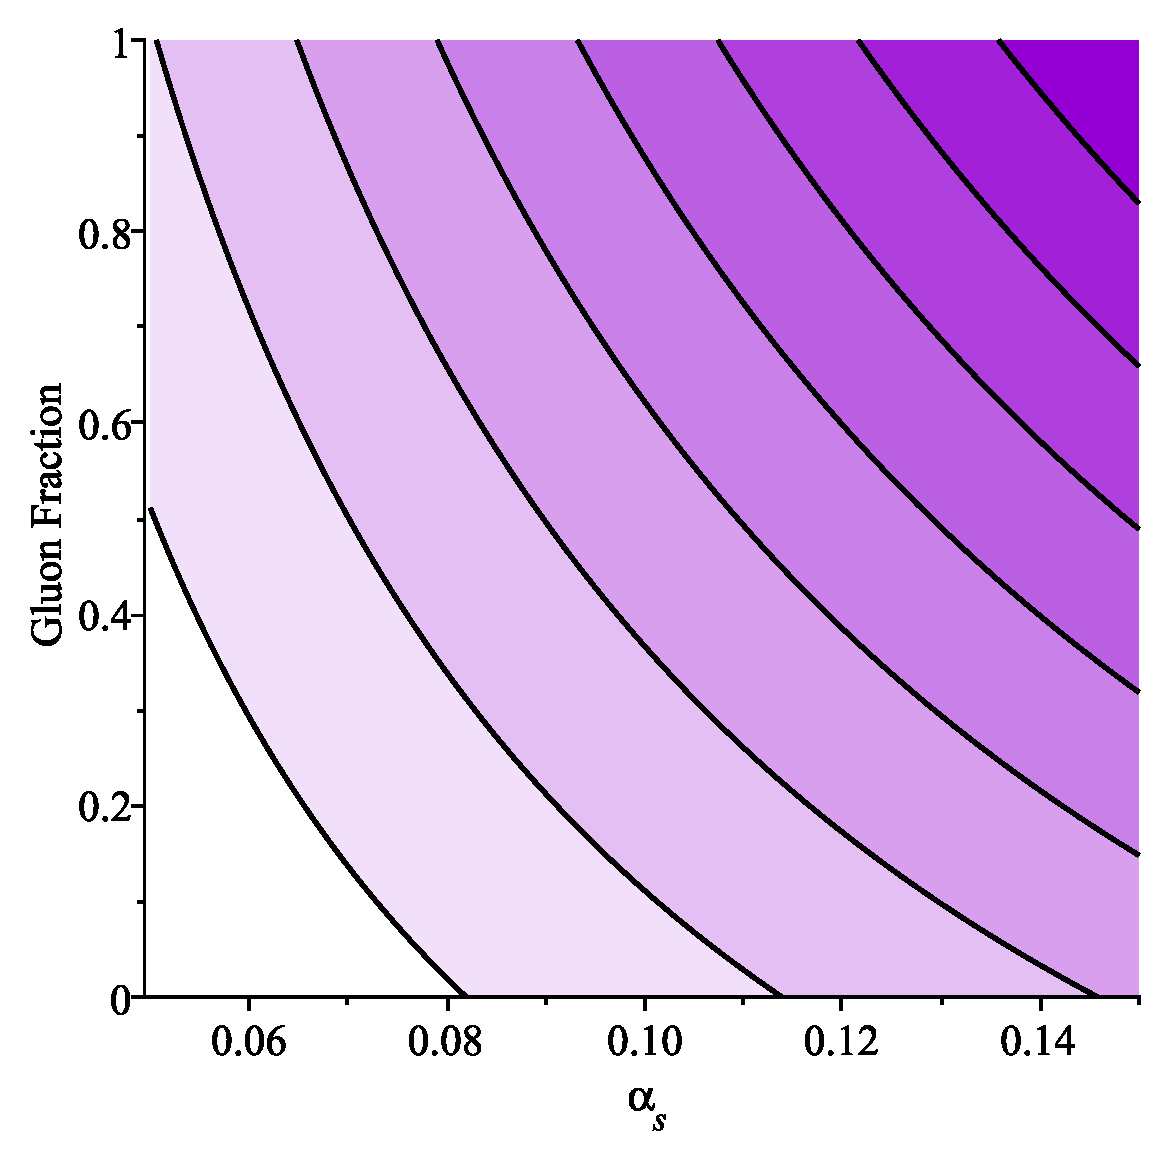
\includegraphics[width = 0.4\columnwidth]{figures/Degeneracy}
\end{center}
\caption{The slope of the probability distribution of $\log(\ecf{2}{2})$ is proportional to $\alpha_s(C_Af_g+C_F(1-f_g))$, which is plotted above.  The degeneracy between $\alpha_s$ and $f_g$ (gluon fraction) are represented by the banana-shaped isocontours. }
\label{fig:analyticbanana}
\end{figure}

A second approach is to simultaneously fit for $\alpha_s$ and the quark/gluon fraction.
%
In the resummation regime, the jet mass distribution only depends on $\alpha_s$ and the quark/gluon fraction.\footnote{At high mass, in the fixed-order regime, there is still residual explicit dependence on PDFs as is the case for the total cross-section.  This regime also suffers from sample-dependent effects where the quark and gluon substructure distributions have residual dependence on the hard process.}
%
Due to the fact that the two fractions must add to unity, this introduces a single additional parameter in the fit (see \Fig{fig:analyticbanana}).
%
The degeneracy between the quark/gluon fraction and $\alpha_s$ is broken by higher order effects.
%
Furthermore, different $\ecf{2}{\alpha}$ have different dependence on $\alpha_s$ and $C_i$ at higher orders.
%
Therefore, the measurement of multiple two-point correlators would allow the degeneracy to be broken.
%
From a theoretical perspective, this significantly complicates the analysis, since it would require precise
predictions to be made for the joint distribution of multiple two-point correlators.


In our fitting study in \Sec{sec:ben_study}, we consider both of the above approaches.
%
It would be interesting to develop other approaches to disentangling the quark and gluon fractions and $\alpha_s$.
%
Without some kind of conceptual breakthrough, though, we expect that the quark/gluon fraction will be a limiting aspect of $\alpha_s$ extractions from jet substructure at the LHC.

%%%%%%%%%%%%%%%%%%%%%%%%%%%
\subsection{Normalized vs.\ Unnormalized Distributions}
%%%%%%%%%%%%%%%%%%%%%%%%%%%

In addition to the complication of quark and gluon fractions, another issue which appears for the extraction of $\alpha_s$ from jet substructure is the issue of normalization.\footnote{We thank Gavin Salam for interesting discussions on this topic.  \jdt{When we get closer to being done, we need to show him a copy of this study.}}
%
Unlike for $e^+e^-$ event shapes, the Born dijet cross section in $pp$ is sensitive to the value of $\alpha_s$.
%
This implies that the rate itself, in particular the absolute quark and gluon jet rates, carries information regarding $\alpha_s$. 

In our studies, we have decided to focus on using normalized distributions.
%
At a conceptual level, this is because we want to perform a true measurement of $\alpha_s$ from jet substructure, which is not dominated by the overall jet rate.
%
But there are two other practical concerns that favor using normalized distributions.

First, it is currently only possible to perform precise measurements of the groomed mass using normalized distributions.
%
Experimentally, the absolute rate is determined by the acceptance from kinematic requirements on the jet $p_\text{T}$.
%
The sophisticated in-situ jet energy scale and resolution program carried out for small-radius jets~\cite{Aad:2014bia,Aaboud:2017jcu,Khachatryan:2016kdb,CMS-DP-2016-020} has not yet reached the same level of maturity for groomed large-radius jets.
%
That said, this is simply a matter of time, and experimental efforts have already started in this direction~\cite{ATLAS-CONF-2017-063}.
%
A key challenge that still remains is to fully understand the correlations in the calibrations and uncertainties between the jet energy and the jet substructure observables.

\begin{figure}[t]
\begin{center}
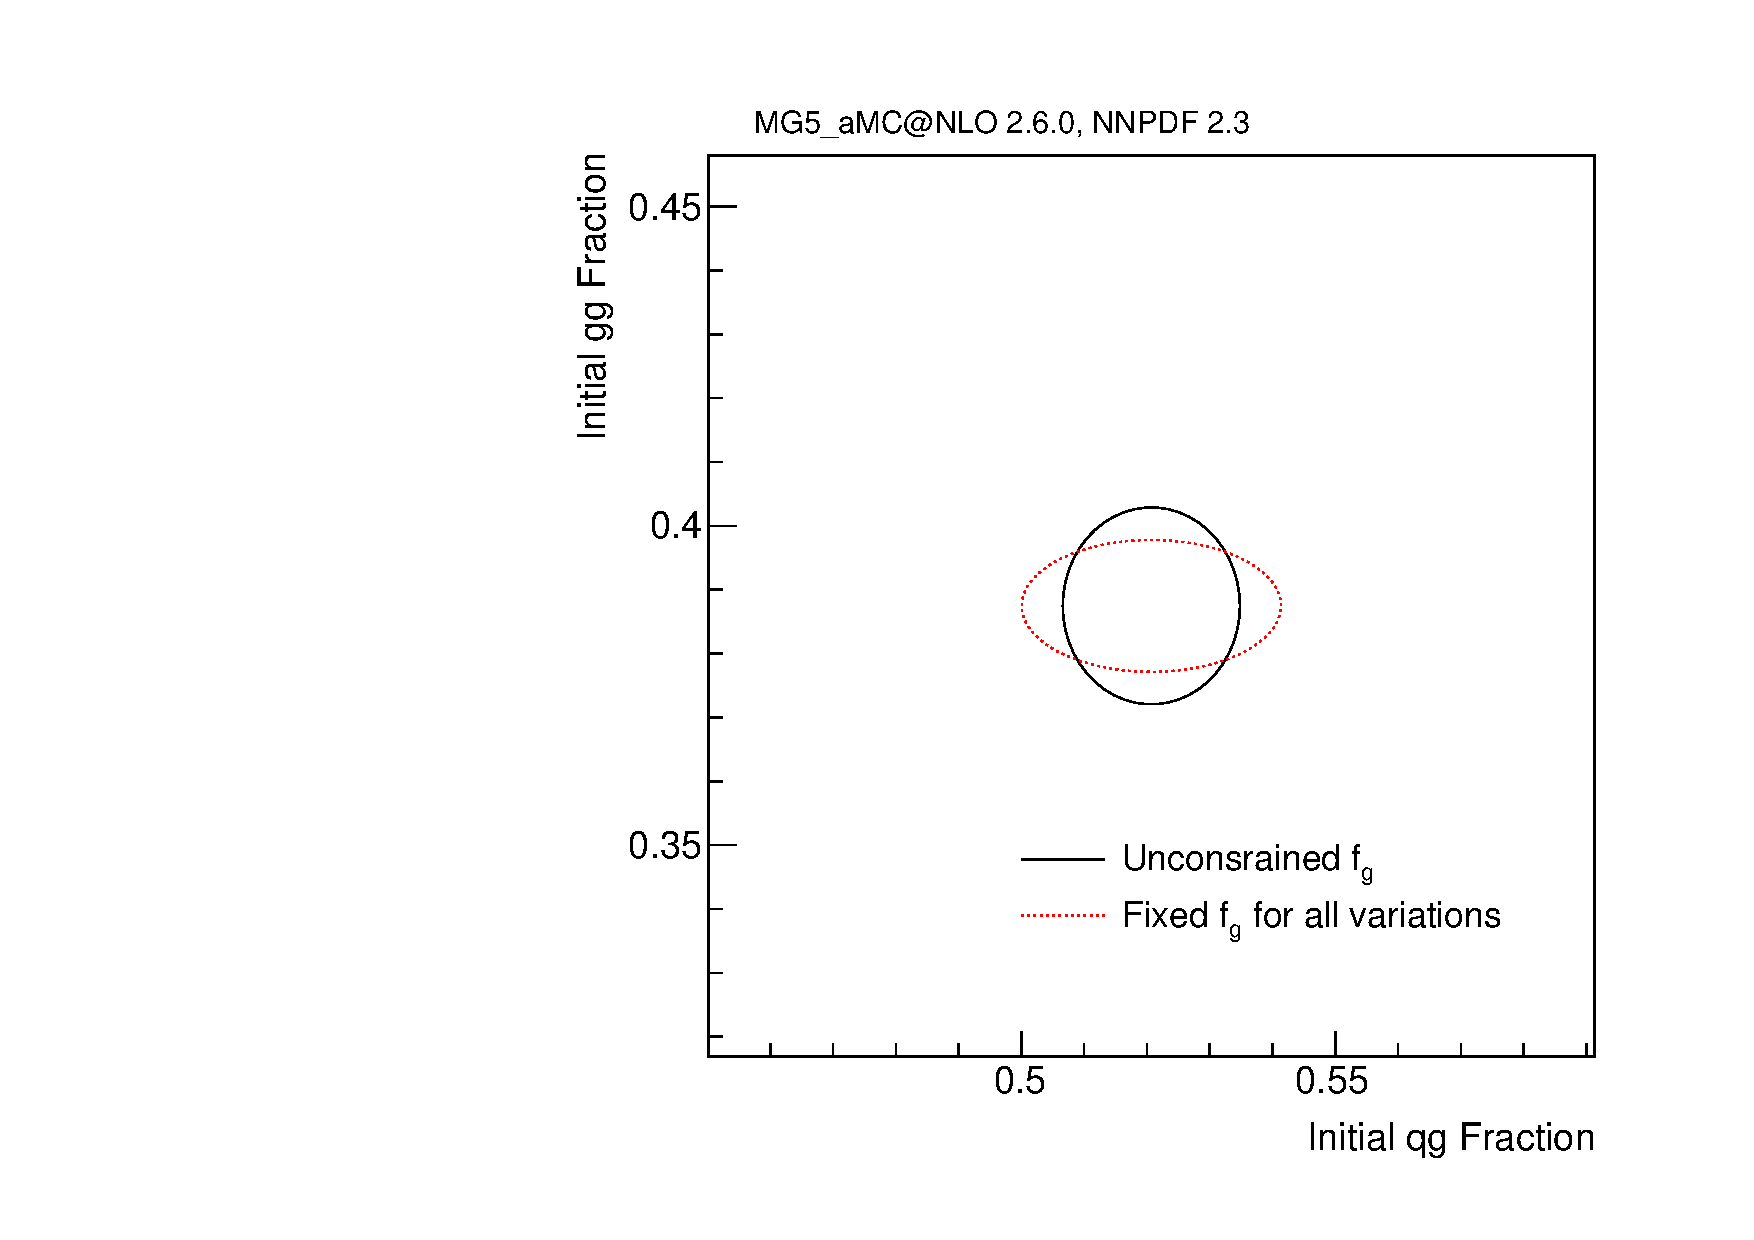
\includegraphics[width = 0.5\columnwidth]{figures/PDFs.pdf}
\end{center}
\caption{The fraction of $qg$ and $gg$ initial states for leading-order dijet production with $p_\text{T}>200$ GeV, simulated at leading order with MG5\_aMC 2.6.0~\cite{Alwall:2014hca} using NNPDF 2.3~\cite{Ball:2012cx}.  The ellipses correspond to the uncertainty from the 100 error PDF sets.  For the red dashed line, the fraction of out-going gluon jets $f_g$ is constrained to be the same for all variations (and equal to the nominal PDF set).}
\label{fig:pdf}
\end{figure}

Second, the use of normalized distributions minimizes the sensitivity to the PDFs.
%
As discussed in \Sec{sec:pertsimplicity}, grooming renders the quark and gluon two-point-correlator distributions universal.
%
Therefore, the measured distribution only depends on the fraction of gluon jets $f_g$ that pass the event selection.
%
In contrast, the total cross-section depends on the relative proportions of all possible partonic initial states, which introduces a source of uncertainty that is not present for the normalized cross-section.
%
For example, the initial state could be one of $qq$, $qg$ or $gg$.
%
The relative proportions can be parameterized by two numbers $f_{qg}$ and $f_{gg}$ where $f_{qg}+f_{gg}=1-f_{qq}$.
%
\Fig{fig:pdf} shows the uncertainty in $f_{qg}$ and $f_{gg}$ from leading-order PDFs.
%
Fixing $f_g$, which carries all of the PDF sensitivity for the shape measurement, has little effect on the uncertainty in $f_{qg}$ and $f_{gg}$.
%
Thus, using unnormalized distributions results in additional PDF sensitivity from also measuring the total cross-section in addition to the shape of the substructure distribution.  \jdt{I tried to reword this last sentence to make it clearer, but I may have gotten the physics wrong.  Please check.}

From the perspective of perturbative accuracy, there is an important issue with using normalized distributions, which is that jet shape observables start at $\cO(\alpha_s)$.
%
Specifically, the slope of the groomed mass distribution is $\cO(\alpha_s)$.
%
This implies that to have an $\cO(\alpha_s^2)$ uncertainty on the slope (as required to gain entry into the PDG world avarage), one needs to have $\cO(\alpha_s^3)$ control, namely the NNLO $2 \to 3$ process for a jet with two constituents.
%
For the case of $e^+e^-$, this level of accuracy has been achieved, where the NNLO corrections to $e^+e^-\to 3$ jets are known and indeed used in the extractions of $\alpha_s$.
%
Due to recent progress in the calculation of the relevant amplitudes, we believe this is a realistic target for jet substructure, but clearly requires substantial further work.

































%%%%%%
